%pbssm
\documentclass[../../main/main.tex]{subfiles}




\begin{document}
\title{Patrol Base Operations as Secure State Machines}


%%%%%%%%%%%%%%%%%%%%% Chapter PB SSM %%%%%%%%%%%%%%%
\chapter{Patrol Base Operations as Secure State Machines} \label{chp:pbssm}
The modularized hierarchy of secure state machines (\glspl{ssm}) consists of many \glspl{ssm}.  The code for all of them can be found in the appendices.  Appendix \ref{app:ssms} contains the pretty-printed \gls{hol} output.  Appendix \ref{aap:ssmScript} contains the \gls{hol} script (raw) code.  These files can also be found in the accompanying files and folders in the folder MasterThesis/HOL/.

Many of the \glspl{ssm} are similar and differ only in the names of the states, commands, and principals.  A representative sample of these is described in this chapter.  The first \gls{ssm}, ssmPB, is a typical example from the hierarchy that uses the OMNI principal and one other principal.  All transitions are sequential.  The next example, ssmConductORP, uses two principals and the OMNI principal.  The third example is ssmPlanPB, which contains the non-sequential conjunction of states.  It does not use the OMNI principal.  All other \glspl{ssm} fit into one of these three patterns.

      %%%%%%%%%%%%%%%%%%% Section ssmPB %%%%%%%%%%%%%
\section{ssmPB: A Typical Example from the Hierarchy}\label{sec:ssmpb}
ssmPB is the top level \gls{ssm}.  It is an example of a typical one-principal\footnote{For the purposes of transitions, the Omni principal isn't thought of as a principal, but a relay.  However, for the purposes of defining principals in \gls{hol}, Omni is included as a principal.} \gls{ssm} that also uses the Omni principal.  A diagram of ssmPB is shown in figure \ref{ssmPBDiagram2}.


\begin{figure}[h!]
\centering
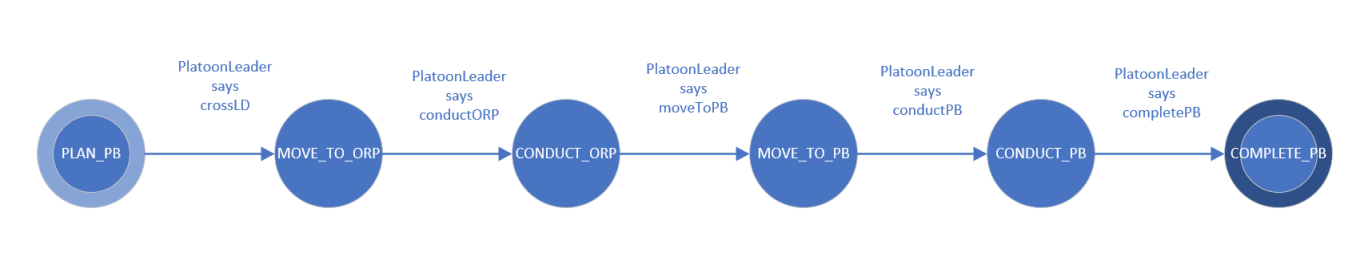
\includegraphics[width=\textwidth]{../figures/ssmPBDiagram}
\caption{\label{ssmPBDiagram2} Top level diagram.}
\end{figure}

ssmPB runs sequentially from the initial state PLAN_PB to the final state COMPLETE_PB.  State transitions require notification from the Omni principal that the state is complete and a request from the Platoon Leader to change states.  Thus, a transition request is a list and has the form\footnote{\textit{stateComplete} and \textit{moveToNextState} are place holders for the actual commands which are defined later.} 
\[\text{\textit{Omni says stateComplete}};\]
\[\text{\textit{PlatoonLeader says moveToNextState}}\]  

The security context reflects this two input requirement.  It authorizes the Platoon Leader on \textit{moveToTheNextState} if the current state is complete. A clause in the security context has the form\footnote{\textit{impf} is the \gls{acl}-\gls{hol} equivalent of "implies"}
\[\text{\textit{stateComplete impf}}\]
\[\text{\textit{PlatoonLeader controls moveToNextState}}\]  

This clause is state dependent because \textit{stateComplete} is specific for the current state.  Thus, there are five statements in the state-dependent security context because there are six states.

There is also a state-independent security context.  This has one clause authorizing the Omni principal on all omniCommands.   It has the form
\[\text{\textit{Omni controls stateComplete}}\]

The \gls{hol} implementation of the datatypes, functions, and theorems are included below.


\subsection{Principals}
The principal datatype is defined in OMNITypeScript.sml.  It has a constructor and one datatype variable.

\HOLFreeVar{principal} = \HOLConst{SR} 'stateRole

\textit{SR} is the type constructor and \textit{'stateRole} is the type variable.  Each \gls{ssm} defines its own principal as a \textit{stateRole}. In ssmPB, the \textit{stateRole} datatype has two principals.

\HOLFreeVar{stateRole} = \HOLConst{PlatoonLeader} \HOLTokenBar{} \HOLConst{Omni}

\subsection{States}
States are also defined in OMNITyrpeScript.sml.

\HOLFreeVar{state} = \HOLConst{ESCs} \HOLTyOp{escState} \HOLTokenBar{} \HOLConst{SLs} 'slState

\textit{'slState} is a state-dependent state which is further defined in each \gls{ssm}.  ssmPB defines six states.

\begin{tabbing}
\HOLFreeVar{slState} = \=\HOLConst{PLAN_PB} \\
					\>\HOLTokenBar{} \HOLConst{MOVE_TO_ORP} \\
					\>\HOLTokenBar{} \HOLConst{CONDUCT_ORP} \\
					\>\HOLTokenBar{} \HOLConst{MOVE_TO_PB}\\
        					\>\HOLTokenBar{} \HOLConst{CONDUCT_PB} \\
					\>\HOLTokenBar{} \HOLConst{COMPLETE_PB}
\end{tabbing}

\subsection{Outputs}
Outputs are defined in OMNITyrpeScript.sml.

\HOLFreeVar{output} = \HOLConst{ESCo} \HOLTyOp{escOutput} \HOLTokenBar{} \HOLConst{SLo} 'slOutput

\HOLConst{SLo} \textit{'slOutput} is the state-dependent output.  It is defined further in each \gls{ssm}.  ssmPB defines seven outputs.

\begin{tabbing}
\HOLFreeVar{slOutput} = \=\HOLConst{PlanPB} \\
					\>\HOLTokenBar{} \HOLConst{MoveToORP} \\
					\>\HOLTokenBar{} \HOLConst{ConductORP} \\
					\>\HOLTokenBar{} \HOLConst{MoveToPB}\\
         				\>\HOLTokenBar{} \HOLConst{ConductPB} \\
					\>\HOLTokenBar{} \HOLConst{CompletePB} \\
					\>\HOLTokenBar{} \HOLConst{unAuthenticated}\\
         				\>\HOLTokenBar{} \HOLConst{unAuthorized}
\end{tabbing}

\textit{unAuthorized} and \textit{unAuthenticated} pertain to \textit{trap} and \textit{discard} transition types, respectively.

\subsection{Commands}
OMNITyrpeScript.sml defines datatypes for all the \glspl{ssm}.

\HOLFreeVar{command} = \HOLConst{ESCc} \HOLTyOp{escCommand} \HOLTokenBar{} \HOLConst{SLc} 'slCommand

\textit{SLc 'slCommand} is further defined in each \gls{ssm}.  ssmPB defines two datatypes for the \textit{slCommand}.

\HOLFreeVar{slCommand} = \HOLConst{PL} \HOLTyOp{plCommand} \HOLTokenBar{} \HOLConst{OMNI} \HOLTyOp{omniCommand}

The \textit{omniCommand} and \textit{plCommand} are further defined in ssmPB.

\begin{tabbing}
\HOLFreeVar{omniCommand} = \=\HOLConst{ssmPlanPBComplete} \\
						\>\HOLTokenBar{} \HOLConst{ssmMoveToORPComplete}\\
            					\>\HOLTokenBar{} \HOLConst{ssmConductORPComplete} \\
						\>\HOLTokenBar{} \HOLConst{ssmMoveToPBComplete}\\
            					\>\HOLTokenBar{} \HOLConst{ssmConductPBComplete} \\
						\>\HOLTokenBar{} \HOLConst{invalidOmniCommand}
\end{tabbing}

\begin{tabbing}
\HOLFreeVar{plCommand} = \=\HOLConst{crossLD} \\
						\>\HOLTokenBar{} \HOLConst{conductORP} \\
						\>\HOLTokenBar{} \HOLConst{moveToPB} \\
						\>\HOLTokenBar{} \HOLConst{conductPB}\\
          					\>\HOLTokenBar{} \HOLConst{completePB} \\
						\>\HOLTokenBar{} \HOLConst{incomplete}
\end{tabbing}

\subsection{Next-State Function}
Each \glsentryshort{ssm} defines its own next-state function.  

\HOLThmTag{ssmPBIntegrated}{PBNS_def}\HOLssmPBIntegratedTheoremsPBNSXXdef

\textit{PBNS} takes a state and a transition (\textit{exec}, \textit{trap}, or \textit{discard}) command list (\textit{x}) as parameters.

The next-state function for ssmPB uses pattern matching and if-then-else statements.  The function first matches the state.  Then, it uses the \textit{getPlCom} function to extract the \HOLFreeVar{plCommand} from the command list \textit{x}. It compares this command to the command on the right.  If they are equal, then the transition occurs.  Otherwise, the state does not change.  

For the \textit{trap} and \textit{discard} transition types (last two lines in the definition), no transition occurs regardless of the command.  Therefore, the command is not checked.  The original state \textit{s} is returned.



\subsection{Next-Output Function}
Each \glsentryshort{ssm} defines its own next-state function. 

\HOLThmTag{ssmPBIntegrated}{PBOut_def}\HOLssmPBIntegratedTheoremsPBOutXXdef

The next-output function behaves similarly to the next-state function.  But, instead of returning the next state, it returns the next output.  The \textit{trap} and \textit{discard} transition types return \textit{unAuthorized} and \textit{unAuthenticated}, respectively, for any command list \textit{x}.

\subsection{Authentication}
The \textit{authenticationTest} function is defined in the parametrizable ssm.  It takes a function as an input and that function takes an input list as an input.  The first function is named \textit{elementTest} in ssm.  It is named \textit{inputOK}\footnote{The function \textit{elementTest} should be thought of as a parameter where \textit{inputOK} specializes that parameter.} in the \glspl{ssm}.

In \gls{hol}, \textit{inputOK} uses the wild card denoted by an underscore "_".  This causes \gls{hol} to generate a lot of additional code when it evaluates the definition.  Both the \gls{hol} definition and the \gls{hol}-generated output for this function are shown below. 


\paragraph*{HOL Definition for inputOK}


\begin{lstlisting}
val inputOK_def =
Define`
(inputOK (((Name PlatoonLeader) says prop (cmd:((slCommand command)option)))
	   :((slCommand command)option, stateRole,'d,'e)Form) = T) /\
(inputOK (((Name Omni)          says prop (cmd:((slCommand command)option)))
	   :((slCommand command)option, stateRole,'d,'e)Form) = T) /\
(inputOK _ = F)`
\end{lstlisting}


The \gls{hol} definition for \textit{inputOK} uses pattern matching.  The first call to \textit{inputOK} matches the input to\\ \centering \textit{(((Name PlatoonLeader) says prop (cmd:((slCommand command)option)))}.\\ \raggedright If it matches, the function returns T for true.  The second call to \textit{inputOK} matches the input to\\
 \centering \textit{(((Name Omni) says prop (cmd:((slCommand command)option)))}.\\  \raggedright If it matches, it returns true.  The last call to \textit{inputOK}  uses the wild card.  This returns false for any other input.

The first two calls to \textit{inputOK} authenticate the PlatoonLeader and Omni principals on any \HOLFreeVar{slCommand}.

\paragraph*{HOL Generated Output for inputOK}

\HOLThmTag{ssmPBIntegrated}{inputOK_def}\HOLssmPBIntegratedTheoremsinputOKXXdef

It is straight forward to prove that any command that is not issued by a principal is rejected.  This follows directly from the definition of \textit{inputOK}.

\HOLThmTag{ssmPBIntegrated}{inputOK_cmd_reject_lemma}\HOLssmPBIntegratedTheoremsinputOKXXcmdXXrejectXXlemma

\subsection{Authorization}
There are two functions for authorization in the parametrizable ssm.  One is state-dependent, the other is not.  

\paragraph*{State-dependent Authorization}
In ssmPB, the state-dependent authorization function is named \textit{secContext}.  \textit{secContext} uses both pattern matching and if-then-else statements. It takes a state and an input list as parameters.

\HOLDfnTag{PBIntegratedDef}{secContext_def}\HOLPBIntegratedDefDefinitionssecContextXXdef

\textit{secContext} uses a helper function named \textit{getOmniCommand} to extract the \HOLFreeVar{omniCommand} from the input list.  It compares this command to the expected command.  If it matches, it returns an implication (\textit{impf}) of the form described in section \ref{sec:ssmpb}.

\paragraph*{HOL Definition for getOmniCommand}
\textit{getOmniCommand} also uses the wildcard "_".  For brevity, only the \gls{hol} definition is presented.

\begin{lstlisting}
val getOmniCommand_def =
Define`
  (getOmniCommand ([]:((slCommand command)option, stateRole, 'd,'e)Form list)
  		      = invalidOmniCommand:omniCommand) /\
  (getOmniCommand (((Name Omni) says prop (SOME (SLc (OMNI cmd))))::xs)
  		      = (cmd:omniCommand)) /\
  (getOmniCommand ((x:((slCommand command)option, stateRole, 'd,'e)Form)::xs)
  		      =  (getOmniCommand xs))`
\end{lstlisting}

\textit{getOmniCommand}  uses pattern matching and recursion.  The first pattern matches the input against the empty list.  This returns \textit{invalidOmniCommand}.  The second pattern matches against a statement of the form \textit{Omni says cmd}.  It returns \textit{cmd}.  The final pattern is a recursive call to \textit{getOmniCommand}.  Thus, if no valid command is present then \textit{invalidOmniCommand} is returned, otherwise the valid \textit{cmd} is returned.


\paragraph*{State-independent Authorization}
The state-independent authorization function \textit{secAuthorization} takes an input list as a parameter.  It uses a helper function called \textit{secHelper}.  \textit{secHelper} calls \textit{getOmniCommand}.  It returns a authorization statement of the form 
\[\text{\textit{Omni controls cmd.}}\]


\HOLDfnTag{PBIntegratedDef}{secAuthorization_def}\HOLPBIntegratedDefDefinitionssecAuthorizationXXdef

\HOLDfnTag{PBIntegratedDef}{secHelper_def}\HOLPBIntegratedDefDefinitionssecHelperXXdef


\subsection{Proved Theorems}\label{ssec:ssmpbproved}
These theorems with their helper lemmas prove the property of complete mediation for each transition in the \gls{ssm}.

\paragraph*{PlatoonLeader_PLAN_PB_exec_justified_thm}
This threorem proves that transition from the PLAN_PB state to the MOVE_TO_ORP state is justified for the following assumptions:
\begin{itemize}
\item The current state is PLAN_PB
\item Omni says ssmPlanPBComplete
\item PlatoonLeader says crossLD
\end{itemize}

Most proofs are similar to this.  Therefore, this first example is described in detail and should be used as a reference for other proofs.

\textit{PlatoonLeader_PLAN_PB_exec_justified_thm} begins by specializing \textit{TR_exec_cmd_rule} described in section \ref{ssec:trrules} of chapter \ref{chp:ssmmodel}.  That rule is repeated here for reference.

\HOLThmTag{ssm}{TR_exec_cmd_rule}\HOLssmTheoremsTRXXexecXXcmdXXrule

Specializing requires use of the ISPECL rule.  This rule takes a list of parameters (lists are enclosed in square brackets) and a theorem (the theorem to be specialized).  

\begin{lstlisting}
val thPlanPB =
  ISPECL
  [``inputOK:((slCommand command)option, stateRole, 'd,'e)Form -> bool``,
  ``secAuthorization :((slCommand command)option, stateRole, 'd,'e)Form list ->
                    ((slCommand command)option, stateRole, 'd,'e)Form list``,
  ``secContext: (slState) ->
       ((slCommand command)option, stateRole, 'd,'e)Form list ->
       ((slCommand command)option, stateRole, 'd,'e)Form list``,
  ``[(Name Omni) says (prop (SOME (SLc (OMNI ssmPlanPBComplete))))
      :((slCommand command)option, stateRole, 'd,'e)Form;
     (Name PlatoonLeader) says (prop (SOME (SLc (PL crossLD))))
      :((slCommand command)option, stateRole, 'd,'e)Form]``,
  ``ins:((slCommand command)option, stateRole, 'd,'e)Form list list``,
  ``(PLAN_PB)``,
  ``outs:slOutput output list trType list``] TR_exec_cmd_rule
\end{lstlisting}

\textit{thPlanPB} is a temporary function used to store an intermediate value. In it, the following values are substituted into the \textit{TR_exec_cmd_rule}.  

\begin{itemize}
\item \textit{inputOK}: substitutes for \textit{elementTest}
\item \textit{secAuthorization}: substitutes for \textit{context}
\item \textit{secContext}: substitutes for \textit{stateInterp}
\item an input list: substitutes for \textit{s}
\item the current state: substitutes for \textit{x}
\item an output list: substitutes for \textit{outs}
\end{itemize}

The \textit{TR_exec_cmd_rule} is already proved in the parametrizable ssm. It is an implication with a hypothesis and a conclusion.  But, with the specialization, it is necessary to prove that the theorem is valid after the authentication and authorization are applied to the input list. To do this, the \textit{thPlanPB} is deconstructed into a hypothesis and conclusion.  Each of these form the basis for a lemma.  The lemmas are then used to prove the overall theorem.

The first lemma begins with the hypothesis of \textit{thPlanPB}. It extracts the hypothesis using the \textit{dest_imp} to destroy the implication and the \textit{fst} function to retain the first part of the result.  

\begin{lstlisting}
fst(dest_imp(concl thPlanPB)))
\end{lstlisting}

The result is a \glsentryshort{hol} term which is used in a tactical proof (backwards proof).
\begin{lstlisting}
val PlatoonLeader_PLAN_PB_exec_lemma =
TAC_PROOF(
  ([],fst(dest_imp(concl thPlanPB))),
REWRITE_TAC[CFGInterpret_def, secContext_def, secAuthorization_def, secHelper_def,
            propCommandList_def,extractPropCommand_def, inputList_def,
	    getOmniCommand_def,
	    MAP,extractInput_def, satList_CONS, satList_nil, GSYM satList_conj]  THEN
PROVE_TAC[Controls,Modus_Ponens])
\end{lstlisting}

The proof consists of a call to the REWRITE_TAC with several definitions passed as parameters (in brackets).  REWRITE_TAC\footnote{See \url{https://hol-theorem-prover.org/kananaskis-11-helpdocs/help/HOLindex.html} for details on \gls{hol} tactics and functions.} rewrites the lemma using the appropriate definition shown in brackets.  The definitions in brackets are defined earlier in this and other chapters. The last line of the proof uses PROVE_TAC, an automatic prover, with the Controls and Modus_Ponens rules.  These rules are described in the \gls{hol} representation of \gls{acl} in chapter \ref{chp:csbdacl} section \ref{sec:aclinhol}.

This lemma is saved as \textit{PlatoonLeader_PLAN_PB_exec_lemma}.  The \gls{hol}-generated output is shown below.

\HOLThmTag{ssmPBIntegrated}{PlatoonLeader_PLAN_PB_exec_lemma}\HOLssmPBIntegratedTheoremsPlatoonLeaderXXPLANXXPBXXexecXXlemma

The next lemma works on the conclusion of \textit{thPlanPB}.  It extracts the conclusion using the \textit{dest_imp} and \textit{snd} rules. 

\begin{lstlisting}
snd(dest_imp(concl thPlanPB)))
\end{lstlisting}

 It is also a tactical proof that uses PROVE_TAC.  PROVE_TAC takes two parameters. The first is the previous lemma and the second is \textit{TR_exec_cmd_rule}.  

\begin{lstlisting}
val PlatoonLeader_PLAN_PB_exec_justified_lemma =
TAC_PROOF(
  ([],snd(dest_imp(concl thPlanPB))),
PROVE_TAC[PlatoonLeader_PLAN_PB_exec_lemma, TR_exec_cmd_rule])
\end{lstlisting}

This lemma is saved as \textit{PlatoonLeader_PLAN_PB_exec_justified_lemma}.  The \gls{hol}-generated output is shown below.

\HOLThmTag{ssmPBIntegrated}{PlatoonLeader_PLAN_PB_exec_justified_lemma}\HOLssmPBIntegratedTheoremsPlatoonLeaderXXPLANXXPBXXexecXXjustifiedXXlemma


With this last lemma, the main theorem is proved using a simple forward proof.  The proof uses the REWRITE_RULE with several theorems including the previous lemma. 

\begin{lstlisting}
val PlatoonLeader_PLAN_PB_exec_justified_thm =
REWRITE_RULE[inputList_def, extractInput_def, MAP, propCommandList_def,
  extractPropCommand_def, PlatoonLeader_PLAN_PB_exec_lemma]
  PlatoonLeader_PLAN_PB_exec_justified_lemma
\end{lstlisting}

The \gls{hol}-generated output is shown below.
\HOLThmTag{ssmPBIntegrated}{PlatoonLeader_PLAN_PB_exec_justified_thm}\HOLssmPBIntegratedTheoremsPlatoonLeaderXXPLANXXPBXXexecXXjustifiedXXthm

With few exceptions, all proofs justifying execution of a command in the \glspl{ssm} follow the same format.

\paragraph*{PlatoonLeader_PLAN_PB_trap_justified_thm}
\textit{PlatoonLeader_PLAN_PB_trap_justified_thm} proves the \textit{trap} transition is justified in the following case
\begin{itemize}
\item current state is PLAN_PB
\item Omni says someOmniCommand and someOmniCommand $\neq$ ssmPlanPBComplete
\item PlatoonLeader says crossLD
\end{itemize}

This is a \textit{trap} because both Omni and PlatoonLeader are authenticated.  But, PlatoonLeader is not authorized to transition to the next state unless Omni says \textit{ssmPlanPBComplete}.



\textit{PlatoonLeader_PLAN_PB_trap_justified_thm} follows the same pattern of implications destruction and lemma proofs.  The difference is that the \textit{TR_trap_cmd_rule} is specialized instead of the \textit{TR_exec_cmd_rule}.  The two lemmas and theorem are shown below as pretty-printed \gls{hol}-generated output.  

\HOLThmTag{ssmPBIntegrated}{PlatoonLeader_PLAN_PB_trap_lemma}\HOLssmPBIntegratedTheoremsPlatoonLeaderXXPLANXXPBXXtrapXXlemma
\HOLThmTag{ssmPBIntegrated}{PlatoonLeader_PLAN_PB_trap_justified_lemma}\HOLssmPBIntegratedTheoremsPlatoonLeaderXXPLANXXPBXXtrapXXjustifiedXXlemma
\HOLThmTag{ssmPBIntegrated}{PlatoonLeader_PLAN_PB_trap_justified_thm}\HOLssmPBIntegratedTheoremsPlatoonLeaderXXPLANXXPBXXtrapXXjustifiedXXthm

\paragraph*{PlatoonLeader_Omni_notDiscard_slCommand_thm}
This theorem proves that if the PlatoonLeader issues an \textit{omniCommand} and Omni issues a \textit{plCommand}, the command is not discarded.  The reason for this is that \textit{plCommand} and \textit{omniCommand} are both \textit{slCommand}s and  \textit{inputOK} authenticates both principals for \textit{slCommand}s.  What this means more generally is that both the PlatoonLeader and Omni are authenticated on any state-level command.

This proof specializes the \textit{TR_discard_cmd_rule}.  This follows a different pattern with no lemmas.  The \gls{hol}-generated output is shown below.

\HOLThmTag{ssmPBIntegrated}{PlatoonLeader_Omni_notDiscard_slCommand_thm}\HOLssmPBIntegratedTheoremsPlatoonLeaderXXOmniXXnotDiscardXXslCommandXXthm

Theorems for each transition are possible. For the most part, they are a cut-n-paste of the theorems above with a few keywords changed.  But, they become repetitive and no new information is gained by showing them here. For completeness, however, they are included in the appendices and file folders as described in the introduction to this chapter.
      %%%%%%%%%%%%%%%%%%% Multiple Principles %% %%%%%%%%%%%
\section{ssmConductORP: Multiple Principals}
ssmConductORP is an example of a \gls{ssm} with more than one principal authorized to execute transitions among states. The diagram is shown in figure \ref{ssmConductORPDiagram2}.


\begin{figure}[h!]
\centering
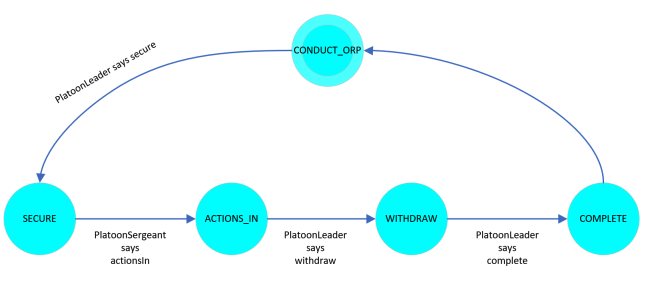
\includegraphics[width=\textwidth]{../figures/ssmConductORPDiagram}
\caption{\label{ssmConductORPDiagram2} Horizontal slice: ConductORP diagram.}
\end{figure}


Other than the number of principals, ssmConductToORP follows the same structure as ssmPB described in the previous section.  

\subsection{Principals}
The principals are defined in the datatype \textit{stateRole}.  There are three principals including Omni.

\HOLFreeVar{stateRole} = \HOLConst{PlatoonLeader} \HOLTokenBar{} \HOLConst{PlatoonSergeant} \HOLTokenBar{} \HOLConst{Omni}

\subsection{States}
States are defined as \HOLFreeVar{slState}.  The names differ only slightly from the diagram but are straight forward.  
\begin{tabbing}
\HOLFreeVar{slState} = \=\HOLConst{CONDUCT_ORP} \\
					\>\HOLTokenBar{} \HOLConst{SECURE} \\
					\>\HOLTokenBar{} \HOLConst{ACTIONS_IN} \\
					\>\HOLTokenBar{} \HOLConst{WITHDRAW}\\
        					\>\HOLTokenBar{} \HOLConst{COMPLETE}
\end{tabbing}

\subsection{Outputs}
Outputs are named similarly to ssmPB outputs.

\begin{tabbing}
\HOLFreeVar{slOutput} = \=\HOLConst{ConductORP} \\
					\>\HOLTokenBar{} \HOLConst{Secure} \\
					\>\HOLTokenBar{} \HOLConst{ActionsIn} \\
					\>\HOLTokenBar{} \HOLConst{Withdraw} \\
					\>\HOLTokenBar{} \HOLConst{Complete}\\
         				\>\HOLTokenBar{} \HOLConst{unAuthenticated} \\
					\>\HOLTokenBar{} \HOLConst{unAuthorized}\end{tabbing}

\subsection{Commands}
The \textit{slCommand} datatype defines three datatype variables, one for each principal.  Each are further defined.
\begin{tabbing}
\HOLFreeVar{slCommand} =\=\HOLConst{PL} \HOLTyOp{plCommand}\\
  						\>\HOLTokenBar{} \HOLConst{PSG} \HOLTyOp{psgCommand}\\
  						\>\HOLTokenBar{} \HOLConst{OMNI} \HOLTyOp{omniCommand}
\end{tabbing}

\textit{plCommand} defines the PlatoonLeader commands.
\begin{tabbing}
\HOLFreeVar{plCommand} = \=\HOLConst{secure} \\
						\>\HOLTokenBar{} \HOLConst{withdraw} \\
						\>\HOLTokenBar{} \HOLConst{complete} \\
						\>\HOLTokenBar{} \HOLConst{plIncomplete}
\end{tabbing}

\textit{psgCommand} defines the PlatoonSergeant commands.
\begin{tabbing}
\HOLFreeVar{psgCommand} = \HOLConst{actionsIn} \HOLTokenBar{} \HOLConst{psgIncomplete}
\end{tabbing}

\textit{omniCommand} defines the Omni commands.
\begin{tabbing}
\HOLFreeVar{omniCommand} = \=\HOLConst{ssmSecureComplete} \\
						\>\HOLTokenBar{} \HOLConst{ssmActionsInComplete}\\
            					\>\HOLTokenBar{} \HOLConst{ssmWithdrawComplete} \\
						\>\HOLTokenBar{} \HOLConst{invalidOmniCommand}
\end{tabbing}



\subsection{Next-State Function}
The next-state function follows the same pattern as for ssmPB.  The only difference is that one of the transitions requires a \textit{psgCommand} instead of a \textit{plCommand}.  This is the transition from SECURE to ACTIONS_IN.

\HOLThmTag{ssmConductORP}{conductORPNS_def}\HOLssmConductORPTheoremsconductORPNSXXdef

The next-state function requires two helper functions just as the next-state function for ssmPB.  These are \textit{getPlCom} and \textit{getPsgCom}.  The former extracts PlatoonLeader commands and the later extracts PlatoonSergeant commands.  They both use the "_" as a wild card.  The \gls{hol} definition for both functions is shown below.
\begin{lstlisting}
val getPlCom_def =
Define`
  (getPlCom ([]:((slCommand command)option)list)
  		      = plIncomplete:plCommand) /\
  (getPlCom (SOME (SLc (PL cmd)):(slCommand command)option::xs)
  		      = cmd:plCommand) /\
  (getPlCom (_::(xs :(slCommand command)option list))
  		      =  (getPlCom xs))`

val getPsgCom_def =
Define`
  (getPsgCom ([]:((slCommand command)option)list)
  		      = psgIncomplete:psgCommand) /\
  (getPsgCom (SOME (SLc (PSG cmd)):(slCommand command)option::xs)
  		      = cmd:psgCommand) /\
  (getPsgCom (_::(xs :(slCommand command)option list))
  		      =  (getPsgCom xs))`
 \end{lstlisting}


\subsection{Next-Output Function}
The next-output function follows the same pattern as the next-state function.  It returns outputs instead of states.

\HOLThmTag{ssmConductORP}{conductORPOut_def}\HOLssmConductORPTheoremsconductORPOutXXdef

\subsection{Authentication}
Authentication uses the \textit{inputOK} function.  It is the same function as the ssmPB \textit{inputOK} except that it adds an additional pattern matching to authenticate the PlatoonSergeant.

\begin{lstlisting}
val inputOK_def =
Define
`(inputOK
 ((Name PlatoonLeader) says (prop  (cmd:(slCommand command)option))
 	:((slCommand command)option,stateRole,'d,'e)Form) = T) /\
 (inputOK
 ((Name PlatoonSergeant) says (prop  (cmd:(slCommand command)option))
 	:((slCommand command)option,stateRole,'d,'e)Form) = T) /\
 (inputOK
 ((Name Omni) says (prop (cmd:(slCommand command)option))
  	:((slCommand command)option,stateRole,'d,'e)Form) = T) /\
 (inputOK _= F)`
 \end{lstlisting}

It is straight forward to prove that any command that is not issued by a principal is rejected.  This follows directly from the definition of \textit{inputOK}.

\HOLThmTag{ssmConductORP}{inputOK_cmd_reject_lemma}\HOLssmConductORPTheoremsinputOKXXcmdXXrejectXXlemma


\subsection{Authorization}
As in ssmPB and all \glspl{ssm}, there is a state-dependent and state-independent authorization function.

\paragraph*{State-dependent Authorization}
Like ssmPB, the state-dependent authorization function is named \textit{secContext}.  It takes a state and an input list as parameters.  It returns an authorization statement.  It follows the same logic as \textit{secContext} in ssmPB.

\HOLDfnTag{ConductORPDef}{secContext_def}\HOLConductORPDefDefinitionssecContextXXdef

\textit{secContext} in ssmConductORP uses the exact same \textit{getOmniCommand} function. It is repeated here as a reference.



\begin{lstlisting}
val getOmniCommand_def =
Define`
  (getOmniCommand ([]:((slCommand command)option, stateRole, 'd,'e)Form list)
  		      = invalidOmniCommand:omniCommand) /\
  (getOmniCommand (((Name Omni) says prop (SOME (SLc (OMNI cmd))))::xs)
  		      = (cmd:omniCommand)) /\
  (getOmniCommand ((x:((slCommand command)option, stateRole, 'd,'e)Form)::xs)
  		      =  (getOmniCommand xs))`
\end{lstlisting}

\paragraph*{State-independent Authorization}
Like ssmPB, the state-independent authorization function is named \textit{secAuthorization}.  It takes only an input list as a parameter.  This is the exact same \textit{secAuthorization} as in ssmPB. It also uses the exact same \textit{secHelper} function as ssmPB.  It is repeated here as a reference.
 

\HOLDfnTag{ConductORPDef}{secAuthorization_def}\HOLConductORPDefDefinitionssecAuthorizationXXdef

\HOLDfnTag{ConductORPDef}{secHelper_def}\HOLConductORPDefDefinitionssecHelperXXdef


\subsection{Proved Theorems}
These theorems follow those in section \ref{ssec:ssmpbproved} for ssmPB.  There are few changes and thus detailed explanation of the proof is omitted.  The pretty-printed \gls{hol}-generated output is included here.

\paragraph*{PlatoonSergeant_SECURE_exec_justified_thm}
This theorem justifies transition from the SECURE state to the ACTIONS_IN  state.  The authenticated principal is the PlatoonSergeant.  This theorem specializes the \textit{TR_exec_cmd_rule}.  The two lemmas and theorem are shown below.

\HOLThmTag{ssmConductORP}{PlatoonSergeant_SECURE_exec_lemma}\HOLssmConductORPTheoremsPlatoonSergeantXXSECUREXXexecXXlemma
\HOLThmTag{ssmConductORP}{PlatoonSergeant_SECURE_exec_justified_lemma}\HOLssmConductORPTheoremsPlatoonSergeantXXSECUREXXexecXXjustifiedXXlemma
\HOLThmTag{ssmConductORP}{PlatoonSergeant_SECURE_exec_justified_thm}\HOLssmConductORPTheoremsPlatoonSergeantXXSECUREXXexecXXjustifiedXXthm

\paragraph*{PlatoonLeader_ACTIONS_IN_exec_justified_thm}
This theorem justifies transition from the ACTIONS_IN state to the WITHDRAW state.  The authenticated principal is the PlatoonLeader.  This theorem specializes the \textit{TR_exec_cmd_rule}.  The two lemmas and theorem are shown below.

\HOLThmTag{ssmConductORP}{PlatoonLeader_ACTIONS_IN_exec_lemma}\HOLssmConductORPTheoremsPlatoonLeaderXXACTIONSXXINXXexecXXlemma
\HOLThmTag{ssmConductORP}{PlatoonLeader_ACTIONS_IN_exec_justified_lemma}\HOLssmConductORPTheoremsPlatoonLeaderXXACTIONSXXINXXexecXXjustifiedXXlemma
\HOLThmTag{ssmConductORP}{PlatoonLeader_ACTIONS_IN_exec_justified_thm}\HOLssmConductORPTheoremsPlatoonLeaderXXACTIONSXXINXXexecXXjustifiedXXthm

\paragraph*{PlatoonLeader_ACTIONS_IN_trap_justified_thm}
This theorem justifies trapping the transition from the ACTIONS_IN state to the WITHDRAW state.  The authenticated principal is the PlatoonLeader.  But, in this case, Omni does not issue the command \textit{ssmActionsInComplete}.  Therefore, the transition is not authorized.  This theorem specializes the \textit{TR_trap_cmd_rule}.  The two lemmas and theorem are shown below.

\HOLThmTag{ssmConductORP}{PlatoonLeader_ACTIONS_IN_trap_lemma}\HOLssmConductORPTheoremsPlatoonLeaderXXACTIONSXXINXXtrapXXlemma
\HOLThmTag{ssmConductORP}{PlatoonLeader_ACTIONS_IN_trap_justified_lemma}\HOLssmConductORPTheoremsPlatoonLeaderXXACTIONSXXINXXtrapXXjustifiedXXlemma
\HOLThmTag{ssmConductORP}{PlatoonLeader_ACTIONS_IN_trap_justified_thm}\HOLssmConductORPTheoremsPlatoonLeaderXXACTIONSXXINXXtrapXXjustifiedXXthm


As with ssmPlanPB, the other theorems are included in the appendices and files.
      %%%%%%%%%%%%%%%%%%% ssmPlanPB %%%%%%%%%%%%%%%%
\section{ssmPlanPB: Non-sequential Transitions}
The ssmPlanPB \gls{ssm} does not use the Omni principal but does use a "sort-of" non-sequential progression through states.  To minimize the complexity of the model, the three states that are non-sequential are represented as "virtual states" whose completion is noted as input to the command to transition from the state before them to the state after them.  Figure \ref{ssmPlanPBDiagram2a} is a diagram of this \gls{ssm}.

\begin{figure}[h!]
\centering
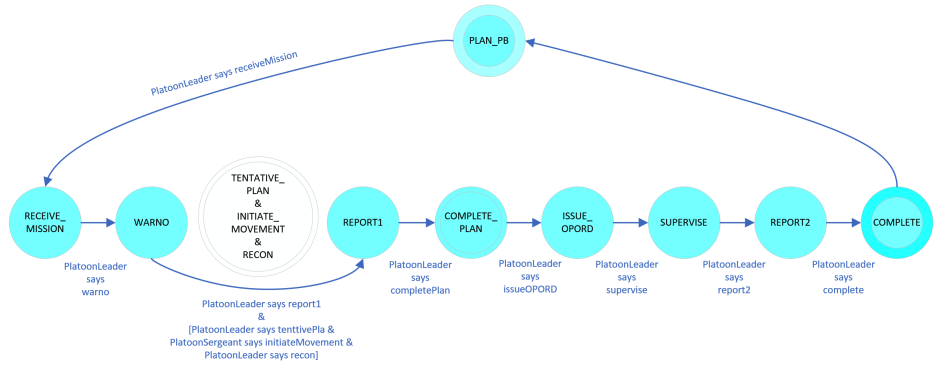
\includegraphics[width=\textwidth]{../figures/ssmPlanPBDiagram}
\caption{\label{ssmPlanPBDiagram2a} Horizontal slice: PlanPB diagram.}
\end{figure}

The three non-sequential states are hidden in the white circle in the diagram.  They are TENTATIVE_PLAN, INITIATE_MOVEMENT, and RECON. These three states may be completed in any order, but all three must be completed before progressing to the next state REPORT1.  

To handle this, the three non-sequential states are combined into one "virtual state."  Completion of these states must preceded transition from the WARNO state to the REPORT1 state.  Completion is indicated by the following three \gls{acl} statements 
\[\text{\textit{PlatoonLeader says tentativePlan}}\]
\[\text{\textit{PlatoonSergeant says initiateMovement}}\]
\[\text{\textit{PlatoonLeader says recon}}\]


when combined with a request from the PlatoonLeader to transition to the REPORT1 state, the input (a list of inputs) for this transition is
\[\text{\textit{PlatoonLeader says tentativePlan}  }\]
\[\text{\textit{PlatoonSergeant says initiateMovement}  }\]
\[\text{\textit{PlatoonLeader says recon}}\]
\[\text{\textit{PlatoonLeader says report1}}\]

The security policy handles this with the following implication
\[\text{\textit{tentativePlan} andf  }\]
\[\text{\textit{initiateMovement} andf  }\]
\[\text{\textit{recon} impf}\]
\[\text{\textit{PlatoonLeader controls recon}}\]

The remaining details of this implementation follow.
\subsection{Principals}
The planning phase \gls{ssm} has two principals: PlatoonLeader and PlatoonSergeant.  These are defined in the \HOLFreeVar{stateRole} datatype.

\HOLFreeVar{stateRole} = \HOLConst{PlatoonLeader} \HOLTokenBar{} \HOLConst{PlatoonSergeant}

\subsection{States}
There are 12 states.  But, TENTATIVE_PLAN, INITIATE_MOVEMENT, and RECON are virtual states and not used in the next-state and next-output functions.

\begin{tabbing}
\parskip=8pt
\HOLFreeVar{slState} = \=\HOLConst{PLAN_PB} \\
				\>\HOLTokenBar{} \HOLConst{RECEIVE_MISSION} \\
				\>\HOLTokenBar{} \HOLConst{WARNO} \\
				\>\HOLTokenBar{} \HOLConst{TENTATIVE_PLAN}\\
        				\>\HOLTokenBar{} \HOLConst{INITIATE_MOVEMENT} \\
				\>\HOLTokenBar{} \HOLConst{RECON} \\
				\>\HOLTokenBar{} \HOLConst{REPORT1} \\
				\>\HOLTokenBar{} \HOLConst{COMPLETE_PLAN}\\
        				\>\HOLTokenBar{} \HOLConst{OPOID} \\
				\>\HOLTokenBar{} \HOLConst{SUPERVISE} \\
				\>\HOLTokenBar{} \HOLConst{REPORT2} \\
				\>\HOLTokenBar{} \HOLConst{COMPLETE}
\parskip=18pt
\end{tabbing}

\subsection{Output}
There are 14 outputs.  But, \textit{PlanPB}, \textit{TentativePlan}, \textit{InitiateMovement}, and \textit{Recon} are not used in the next-output function.  The \textit{unAuthorized} output is returned for trapped commands.  The \textit{unAuthenticated} output is returned for discarded commands.

\begin{tabbing}
\parskip=8pt
\HOLFreeVar{slOutput} =  \=\HOLConst{PlanPB} \\
					\>\HOLTokenBar{} \HOLConst{ReceiveMission} \\
					\>\HOLTokenBar{} \HOLConst{Warno} \\
					\>\HOLTokenBar{} \HOLConst{TentativePlan}\\
         				\>\HOLTokenBar{} \HOLConst{InitiateMovement} \\
					\>\HOLTokenBar{} \HOLConst{Recon} \\
					\>\HOLTokenBar{} \HOLConst{Report1} \\
					\>\HOLTokenBar{} \HOLConst{CompletePlan}\\
         				\>\HOLTokenBar{} \HOLConst{Opoid} \\
					\>\HOLTokenBar{} \HOLConst{Supervise} \\
					\>\HOLTokenBar{} \HOLConst{Report2} \\
					\>\HOLTokenBar{} \HOLConst{Complete}\\
         				\>\HOLTokenBar{} \HOLConst{unAuthenticated} \\
					\>\HOLTokenBar{} \HOLConst{unAuthorized}
\parskip=18pt
\end{tabbing}

\subsection{Commands}
The \textit{slCommand} datatype for this \gls{ssm} is defined below.

\HOLFreeVar{slCommand} = \HOLConst{PL} \HOLTyOp{plCommand} \HOLTokenBar{} \HOLConst{PSG} \HOLTyOp{psgCommand}

The two datatypes for \textit{plCommand} and \textit{psgCommand} represent the PlatoonLeader and PlatoonSergeant commands, respectively. These are defined below.

\begin{tabbing}
\parskip=8pt
\HOLFreeVar{plCommand} = \=\HOLConst{receiveMission} \\
					     \>\HOLTokenBar{} \HOLConst{warno} \\
					     \>\HOLTokenBar{} \HOLConst{tentativePlan} \\
					     \>\HOLTokenBar{} \HOLConst{recon}\\
          				     \>\HOLTokenBar{} \HOLConst{report1} \\
				     	     \>\HOLTokenBar{} \HOLConst{completePlan} \\
					     \>\HOLTokenBar{} \HOLConst{opoid} \\
					     \>\HOLTokenBar{} \HOLConst{supervise} \\
					     \>\HOLTokenBar{} \HOLConst{report2}\\
          				     \>\HOLTokenBar{} \HOLConst{complete} \\
				     	     \>\HOLTokenBar{} \HOLConst{plIncomplete} \\
					     \>\HOLTokenBar{} \HOLConst{invalidPlCommand}
\parskip=18pt
\end{tabbing}

\begin{tabbing}
\parskip=8pt
\HOLFreeVar{psgCommand} = \=\HOLConst{initiateMovement} \\
						\>\HOLTokenBar{} \HOLConst{psgIncomplete}\\
           					\>\HOLTokenBar{} \HOLConst{invalidPsgCommand}
\parskip=18pt
\end{tabbing}

Providing each principal with her own set of commands simplifies the authentication and authorization functions.


\subsection{Next-State Function}
The next-state function is defined similarly to those defined for previously described \glspl{ssm}.  

\HOLThmTag{ssmPlanPB}{planPBNS_def}\HOLssmPlanPBTheoremsplanPBNSXXdef

Five functions are defined (see below) to extract the command from the input list.  These are \textit{getRecon}, \textit{getTentativePlan}, \textit{getReport}, \textit{getInitMove}, and \textit{getPlCom}.  Each of these functions takes an input list as a parameter and returns a command with its option type.  For the sake of brevity, only \textit{getRecon} is shown below.  The other functions are similar.

\paragraph*{HOL Definition for getRecon}...

\begin{lstlisting}
val getRecon_def = Define `
    (getRecon ([]:((slCommand command)option, stateRole, 'd,'e)Form list) =
    	      [NONE]) /\
    (getRecon ((Name PlatoonLeader) says (prop (SOME (SLc (PL recon))))
               :((slCommand command)option, stateRole, 'd,'e)Form::xs)
    	      	        = [SOME (SLc (PL recon)):(slCommand command)option]) /\
    (getRecon (_::xs) = getRecon xs)`
\end{lstlisting}

\subsection{Next-Output Function}
The next-output function is defined similarly to those defined for previously described \glspl{ssm}.

\HOLThmTag{ssmPlanPB}{planPBOut_def}\HOLssmPlanPBTheoremsplanPBOutXXdef


\subsection{Authentication}
Authentication for this \gls{ssm} is the same as for the previously described \glspl{ssm}.

\paragraph*{HOL Definition for inputOK}

\begin{lstlisting}
val inputOK_def = Define
`(inputOK
	(((Name PlatoonLeader) says (prop  (cmd:((slCommand command)option))))
	       :((slCommand command)option, stateRole, 'd,'e)Form) = T)  /\
(inputOK
	(((Name PlatoonSergeant) says (prop  (cmd:((slCommand command)option))))
	       :((slCommand command)option, stateRole, 'd,'e)Form) = T)  /\
(inputOK _ = F)`
\end{lstlisting}

It is straight forward to prove that any command that is not requested by a principal is false.

\begin{lstlisting}
val inputOK_cmd_reject_lemma =
TAC_PROOF(
  ([],
   ``!cmd. ~(inputOK
   	   ((prop (SOME cmd)):((slCommand command)option, stateRole, 'd,'e)Form))``),
  PROVE_TAC[inputOK_def])
\end{lstlisting}

\subsection{Authorization}
The two authorization functions are defined below.

\begin{lstlisting}
val secContext_def = Define `
secContext (s:slState) (x:((slCommand command)option, stateRole, 'd,'e)Form list) =
    if (s = WARNO) then
        (if (getRecon         x = [SOME (SLc (PL recon))
                                   :(slCommand command)option] ) /\
	    (getTenativePlan  x = [SOME (SLc (PL tentativePlan))
	    		      	   :(slCommand command)option]) /\
            (getReport        x = [SOME (SLc (PL report1))
	    		      	   :(slCommand command)option]) /\
	    (getInitMove      x = [SOME (SLc (PSG initiateMovement))
	    		      	   :(slCommand command)option])
         then [
	       PL_WARNO_Auth
	        :((slCommand command)option, stateRole, 'd,'e)Form;
		(Name PlatoonLeader) controls prop (SOME (SLc (PL recon)));
		(Name PlatoonLeader) controls prop (SOME (SLc (PL tentativePlan)));
	       (Name PlatoonSergeant) controls prop (SOME (SLc (PSG initiateMovement)))]
	 else [(prop NONE):((slCommand command)option, stateRole, 'd,'e)Form])
    else if ((getPlCom x) = invalidPlCommand)
    	 then [(prop NONE):((slCommand command)option, stateRole, 'd,'e)Form]
	 else [PL_notWARNO_Auth (getPlCom x)]`
\end{lstlisting}

secContext uses \textit{PL_WARNO_Auth} and \textit{PL_notWARNO_Auth}. These are defined below.


\begin{lstlisting}
val PL_WARNO_Auth_def = Define `
    PL_WARNO_Auth =
    ^(impfTermList
    [``(prop (SOME (SLc (PL recon))))
         :((slCommand command)option, stateRole, 'd,'e)Form``,
     ``(prop (SOME (SLc (PL tentativePlan))))
         :((slCommand command)option, stateRole, 'd,'e)Form``,
     ``(prop (SOME (SLc (PSG initiateMovement))))
         :((slCommand command)option, stateRole, 'd,'e)Form``,
     ``(Name PlatoonLeader) controls prop (SOME (SLc (PL report1)))
         :((slCommand command)option, stateRole, 'd,'e)Form``]
     ``:((slCommand command)option, stateRole, 'd,'e)Form``)`
\end{lstlisting}


\begin{lstlisting}
val PL_notWARNO_Auth_def = Define `
    PL_notWARNO_Auth (cmd:plCommand) =
    if (cmd = report1) (* report1 exits WARNO state *)
    then
      (prop NONE):((slCommand command)option, stateRole, 'd,'e)Form
    else
      ((Name PlatoonLeader) says (prop (SOME (SLc (PL cmd)))
       :((slCommand command)option, stateRole, 'd,'e)Form) impf
      (((Name PlatoonLeader) controls prop (SOME (SLc (PL cmd))))
      :((slCommand command)option, stateRole, 'd,'e)Form)) `
\end{lstlisting}

\subsection{Proved Theorems}
Theorems proving complete mediation follow the same format as those for previously described \glspl{ssm}.

\paragraph*{PlatoonLeader_notWARNO_notreport1_exec_plCommand_justified_thm}
This theorem proves that if the state is not WARNO and the \textit{plCommand} is not \textit{report1} then execution of any \textit{plCommand} is justified.  It uses two lemmas and a theorem and follows the same pattern as the the other three-part proofs.  The pretty-printed \gls{hol}-generated output is shown below.

\HOLThmTag{ssmPlanPB}{PlatoonLeader_notWARNO_notreport1_exec_plCommand_lemma}\HOLssmPlanPBTheoremsPlatoonLeaderXXnotWARNOXXnotreportOneXXexecXXplCommandXXlemma

\HOLThmTag{ssmPlanPB}{PlatoonLeader_notWARNO_notreport1_exec_plCommand_justified_lemma}\HOLssmPlanPBTheoremsPlatoonLeaderXXnotWARNOXXnotreportOneXXexecXXplCommandXXjustifiedXXlemma

\HOLThmTag{ssmPlanPB}{PlatoonLeader_notWARNO_notreport1_exec_plCommand_justified_thm}\HOLssmPlanPBTheoremsPlatoonLeaderXXnotWARNOXXnotreportOneXXexecXXplCommandXXjustifiedXXthm

\paragraph*{PlatoonLeader_psgCommand_notDiscard_thm}
This next theorem proves that if the PlatoonLeader issues a \textit{psgCommand} then that command is not discarded.  The reason for this is that the \textit{psgCommand} is an \textit{slCommand}.  In \textit{inputOK}, the PlatoonLeader is authenticated on all \textit{slCommand}s.  (Only unauthenticated requests are discarded.)  This theorem has no lemmas.

\HOLThmTag{ssmPlanPB}{PlatoonLeader_psgCommand_notDiscard_thm}\HOLssmPlanPBTheoremsPlatoonLeaderXXpsgCommandXXnotDiscardXXthm


\paragraph*{PlatoonSergeant_trap_plCommand_justified_thm}
This next theorem proves that if the PlatoonLeader issues a \textit{psgCommand} then that command is trapped.  It specializes the \textit{TR_trap_cmd_rule} with two lemmas and a theorem.

\HOLThmTag{ssmPlanPB}{PlatoonLeader_trap_psgCommand_lemma}\HOLssmPlanPBTheoremsPlatoonLeaderXXtrapXXpsgCommandXXlemma

\HOLThmTag{ssmPlanPB}{PlatoonLeader_trap_psgCommand_justified_lemma}\HOLssmPlanPBTheoremsPlatoonLeaderXXtrapXXpsgCommandXXjustifiedXXlemma

\HOLThmTag{ssmPlanPB}{PlatoonSergeant_trap_plCommand_justified_thm}\HOLssmPlanPBTheoremsPlatoonSergeantXXtrapXXplCommandXXjustifiedXXthm


\paragraph*{PlatoonLeader_WARNO_exec_report1_justified_thm}
This theorem proves that transition from the WARNO to the REPORT1 is justified if the following four statements are supplied.
\begin{itemize}
\item PlatoonLeader says tentativePlan
\item PlatoonSergeant says initiateMovement
\item PlatoonLeader says recon
\item PlatoonLeader says report1
\end{itemize}

It specializes the \textit{TR_exex_cmd_rule} and requires the standard two lemmas and a theorem. 

\HOLThmTag{ssmPlanPB}{PlatoonLeader_WARNO_exec_report1_lemma}\HOLssmPlanPBTheoremsPlatoonLeaderXXWARNOXXexecXXreportOneXXlemma

\HOLThmTag{ssmPlanPB}{PlatoonLeader_WARNO_exec_report1_justified_lemma}\HOLssmPlanPBTheoremsPlatoonLeaderXXWARNOXXexecXXreportOneXXjustifiedXXlemma

\HOLThmTag{ssmPlanPB}{PlatoonLeader_WARNO_exec_report1_justified_thm}\HOLssmPlanPBTheoremsPlatoonLeaderXXWARNOXXexecXXreportOneXXjustifiedXXthm


\paragraph*{PlatoonSergeant_trap_plCommand_justified_thm}
This final theorem proves that the PlatoonSergeant is trapped on all \textit{plCommands}.  This is for the same reason that the PlatoonLeader is trapped on all \textit{psgCommands}.

\HOLThmTag{ssmPlanPB}{PlatoonSergeant_trap_plCommand_lemma}\HOLssmPlanPBTheoremsPlatoonSergeantXXtrapXXplCommandXXlemma

\HOLThmTag{ssmPlanPB}{PlatoonSergeant_trap_plCommand_justified_lemma}\HOLssmPlanPBTheoremsPlatoonSergeantXXtrapXXplCommandXXjustifiedXXlemma

\HOLThmTag{ssmPlanPB}{PlatoonSergeant_trap_plCommand_justified_thm}\HOLssmPlanPBTheoremsPlatoonSergeantXXtrapXXplCommandXXjustifiedXXthm

In concluding this chapter, note that the model here is a first approximation to modeling the patrol base operations.  Some of the proofs may not accurately reflect real patrol base operations.  For example, the Platoon Leader should probably be authorized on ALL commands.  But, we applied the principal of least privilege and restricted transition requests to the responsible principal rather than all who should have been permitted.

The next chapter discusses the results described in the previous chapters.

\end{document}